\documentclass[11pt,twoside]{article}
\usepackage[utf8]{inputenc}
\usepackage[T1]{fontenc}
\usepackage{tabularx}

% Pacchetti per margini, intestazioni, grafica e colori
\usepackage{geometry}
\geometry{
    a4paper,
    total={210mm,297mm},
    left=25mm,
    right=25mm,
    top=30mm,
    bottom=25mm,
    headsep=7mm
}
\usepackage{graphicx}
\usepackage[dvipsnames, table]{xcolor}
\usepackage{fancyhdr}
\usepackage{tocloft}

% Personalizzazione intestazioni e piè di pagina
\pagestyle{fancy}
\fancyhf{}
\lhead{\color{Gray}{\small{Students\&Companies project by Belfiore, Bendetti, Buccheri}}}
\lfoot{\textcolor{Gray}{\small{Copyright © 2024,Belfiore M., Benedetti G., Buccheri G. – All rights reserved}}}
\rfoot{\textcolor{Gray}{\thepage}}
\renewcommand{\headrulewidth}{0pt}

% Configurazione toc
\renewcommand{\cftsecleader}{\cftdotfill{\cftdotsep}}

% Inizio del documento
\begin{document}

% Pagina del titolo
\begin{titlepage}
    \begin{center}
        
\includegraphics[scale=0.5]{Images/PolimiLogo} \\[2cm]
    \end{center}
    
    \begin{center}
        {\color{RoyalBlue}\textbf{\Huge{Software Engineering 2 \\[1cm] Requirements Analysis and Specification Document \\[0.5cm] \textit{Students\&Companies}}}} \\[5cm]
        {\Large Authors: \\ Belfiore Mattia, \\  Benedetti Gabriele,\\ Buccheri Giuseppe.} \\[1cm]
        {\large Academic Year: 2024-2025} \\[0.5cm]
        {\large Version: 1.0} \\[0.5cm]
        {\large Release date: 22/12/2024} \\[2cm]
    \end{center}

    \vfill
    
    \begin{flushright}
        {\footnotesize \textcolor{Gray}{\emph{Copyright © 2024, Belfiore M., Benedetti G., Buccheri G. – All rights reserved.}}}
    \end{flushright}
\end{titlepage}

% Sommario
\clearpage
\tableofcontents
\newpage

% Inizio delle sezioni
\section{Introduction}
\subsection{Purpose}

\subsubsection{Goals}

\subsection{Scope} 

\subsubsection{World Phenomena}
\subsubsection{Shared Phenomena}

\subsection{Definitions, Acronyms, Abbreviations}

\subsection{Revision history}

\subsection{Reference Documents}

\subsection{Document Structure}


\section{Overall Description}

\subsection{Product Perspective}

\subsubsection{Scenarios}
\subsubsection{Class Diagrams}
\subsubsection{State Diagrams}


Figure~\ref{fig:class-diagram} 
\begin{figure}[h!]
    \centering
    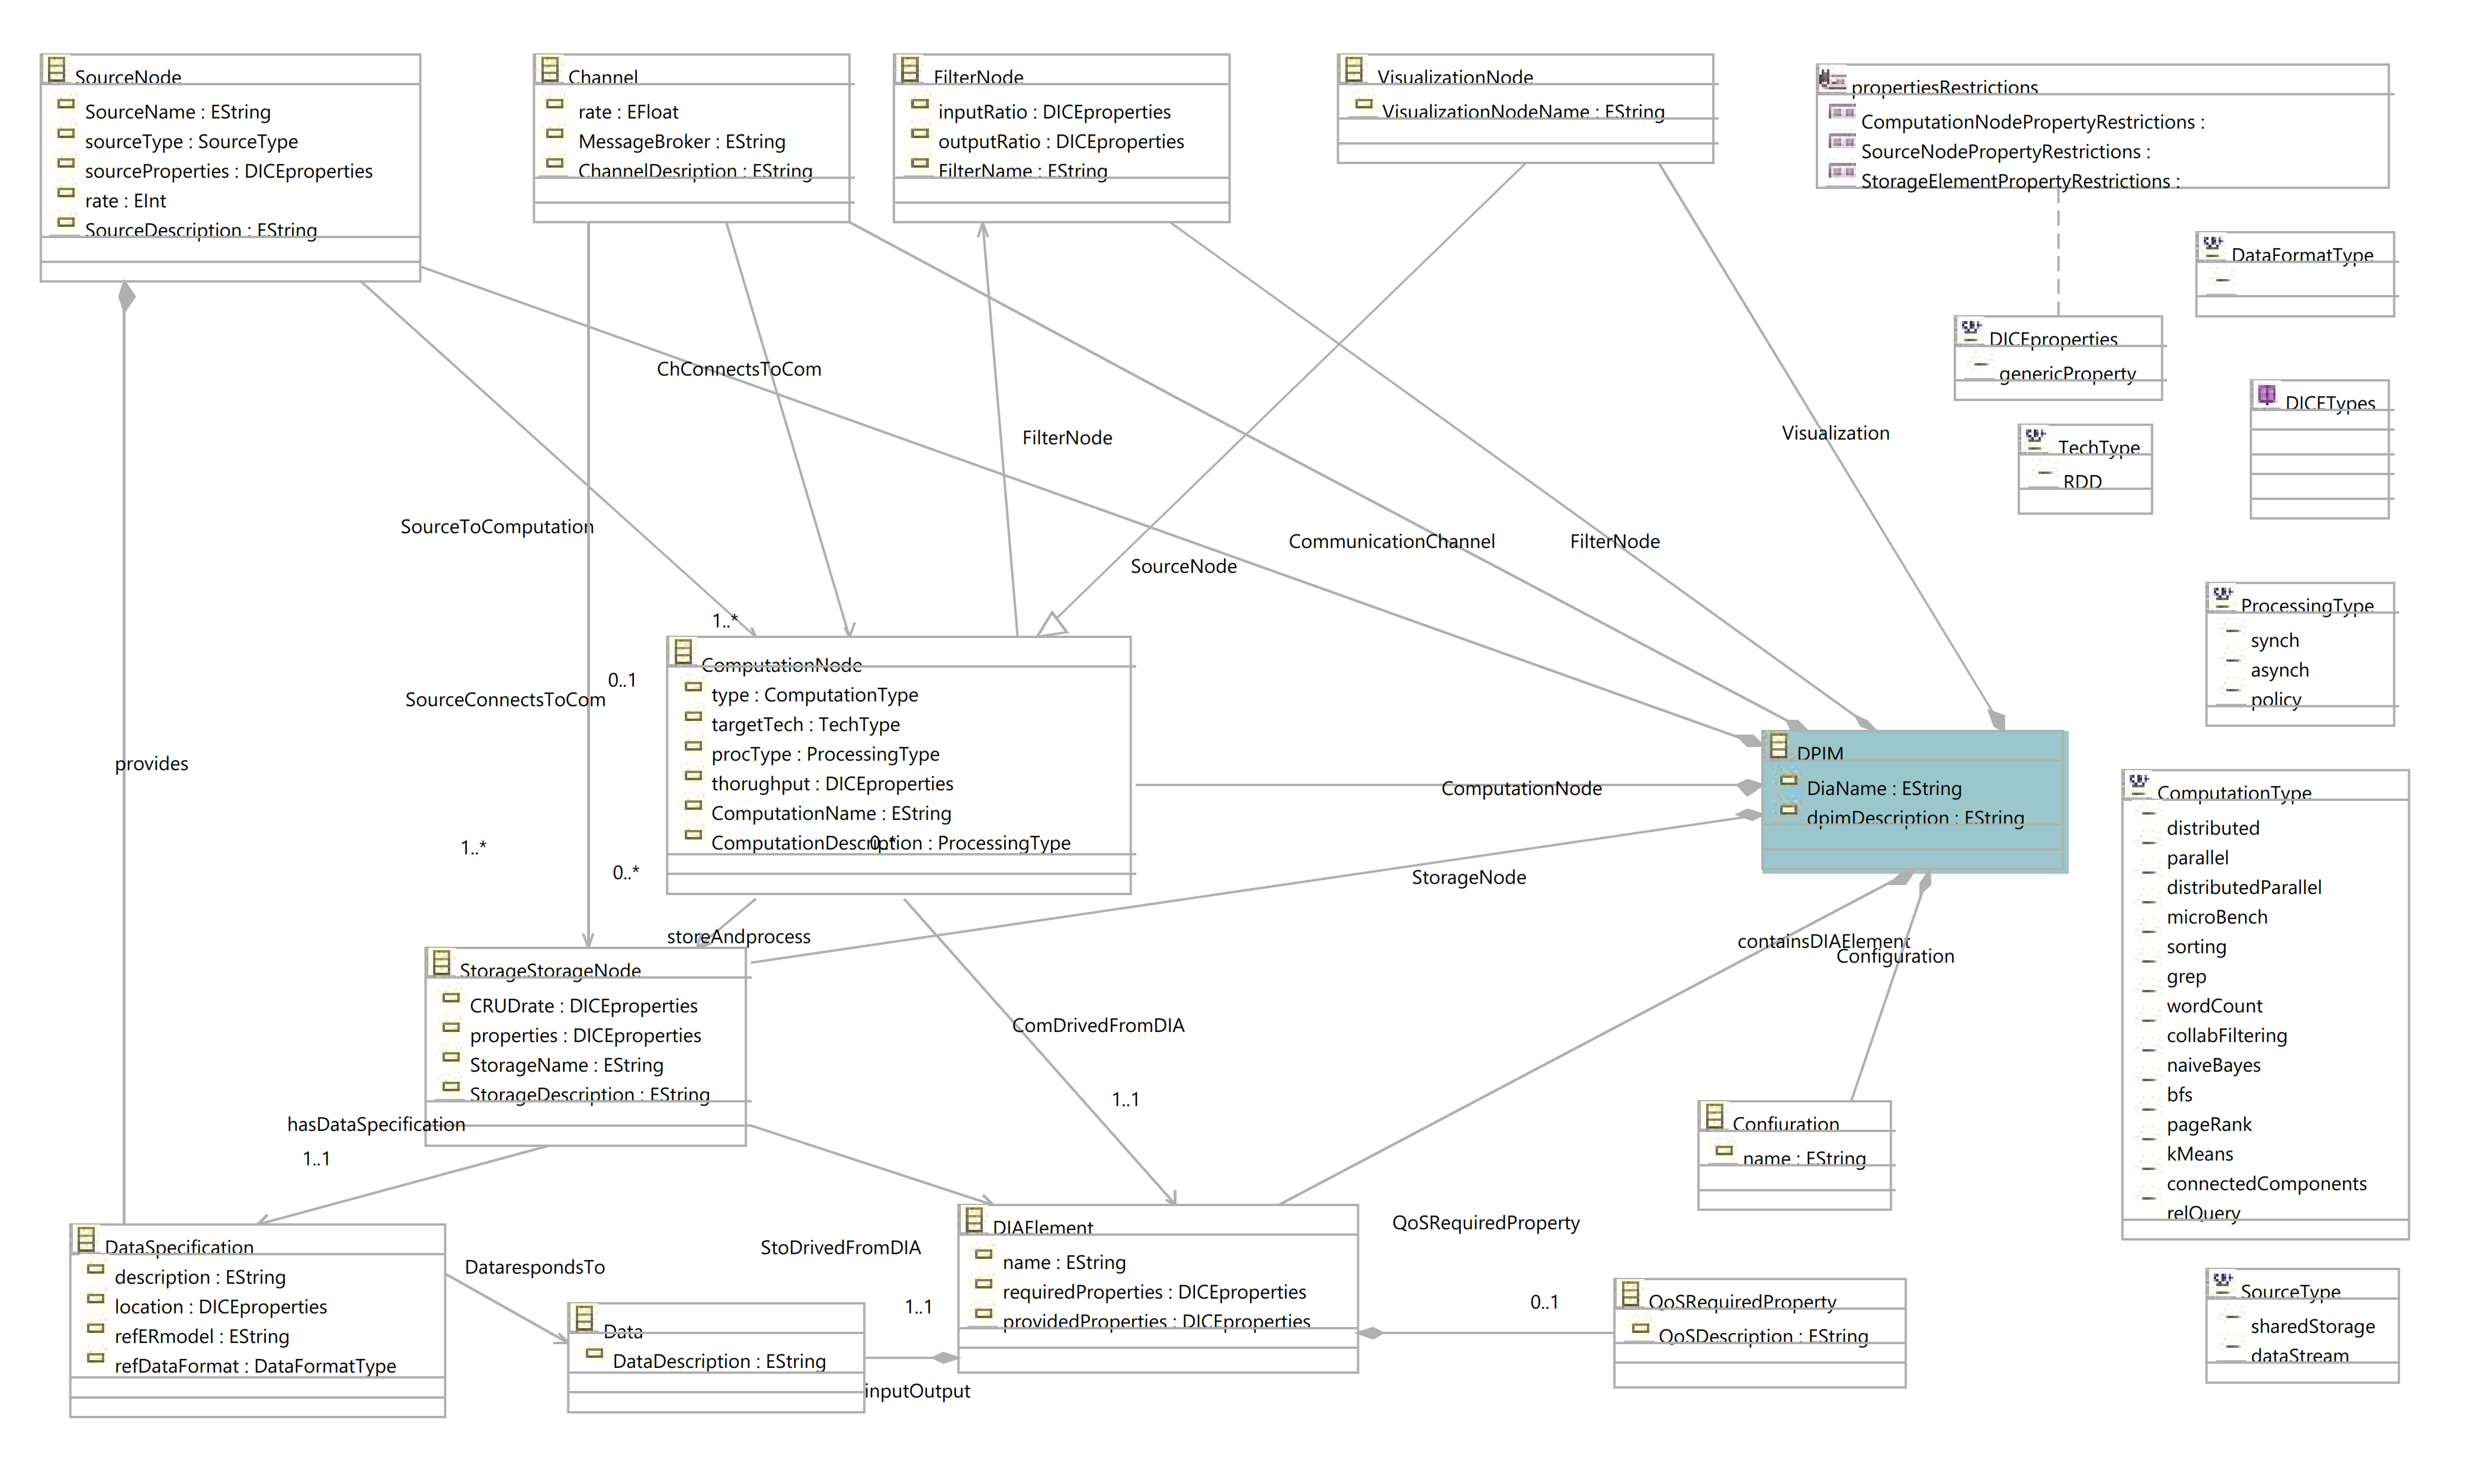
\includegraphics[width=0.8\textwidth]{Images/11.png}
    \caption{High-level Class Diagram}
    \label{fig:class-diagram}
\end{figure}

\subsection{Product Functions}

\subsection{User characteristics}

\subsection{Assumptions, dependencies and constraints}

\subsubsection{Domain Assumptions}

\section{Specific Requirements}

\subsection{External Interface Requirements}

\subsubsection{User interfaces}
\subsubsection{Hardware interfaces}
\subsubsection{Software interfaces}
\subsubsection{Communication interfaces}

\subsection{Functional requirements}

\subsubsection{Requirements}
\subsubsection{Use case diagrams}
\subsubsection{Use case}
\subsubsection{Mapping on goals}

\subsection{Performance requirements}
\subsection{Desgign constraints}

\subsubsection{Standard compliance}
\subsubsection{Hardware limitations}

\subsection{Software systems attributes}
\subsubsection{Reliability}
\subsubsection{Availability}
\subsubsection{Security}
\subsubsection{Maintainability}
\subsubsection{Portability}

\section{Formal Analysis Using Alloy}

\section{Effort Spent}

\noindent\begin{tabular}{|c|c|}

\hline
\textbf{Contributor} & \textbf{Effort (hours)} \\ \hline
Belfiore Mattia & 2 \\ \hline
Benedetti Gabriele & 2 \\ \hline
Buccheri Giuseppe & 2 \\ \hline
Total & 6 \\ \hline
\end{tabular}

\section{References}

\subsection{References}
\subsection{Used Tools}


% Fine del documento
\end{document}
